\documentclass[12pt,a4paper]{article}
 
\usepackage{float}
%für feststellen der figures und tables [H] dranschreiben
\usepackage{units}
%wird so benutzt: 
%\unit[value/Zahl]{dimension/Einheit} oder 
%\unitfrac[value/Zahl]{dimension/Einheit num/Zähler}{dimension/Einheit denum/Nenner} oder
%\nicefrac[fontcommand/Schriftart]{dimension/Einheit num/Zähler}{dimension/Einheit denum/Nenner}
\usepackage[left=2cm,right=2cm,top=2cm,bottom=2cm]{geometry}
\usepackage[utf8]{inputenc}
\usepackage[T1]{fontenc}
\usepackage{lmodern}
\usepackage[ngerman]{babel}
\usepackage{amsmath}
\usepackage{graphicx}
 
\title{Versuch AP8\\ Elektronenstrahlen}
\author{Frederik Strothmann, Henrik Jürgens}
\date{\today}
%niemals zwei überschriften direkt übereinander schreiben, also immer mindestens in einem satz was sinnvolles unter jede überschrift schreiben (bei den versuchen z.B. das versuchsziel) 
\begin{document}
%deckblatt erstellen.
\maketitle
\newpage
\tableofcontents
\newpage
\section{Einleitung}
%einleitung zu dem experiment.
%auf die einstellungen, die vor dem versuch gemacht werden, eingehen oder auf eine anleitung dazu verweisen.
Die Entdeckung der Welleneigenschaften von massebehafteten Teilchen war historisch von größter Bedeutung
für die Entwicklung der Quantenmechanik. Dabei nimmt die Schrödingergleichung als charakteristische Wellengleichung einen besonderen Stellenwert ein, da sie die Grundlage für die nicht-relativistische Quantenmechanik
bildet. In diesem Versuch führen wir zwei Teilexperimente durch, die die Teilchen- bzw. Welleneigenschaften von Elektronen demonstrieren. Mit Hilfe eines Fadenstrahlrohres bestimmen wir die spezifische Ladung e/m eines Elektrons, das im homogenen Magnetfeld eines Helmholtzspulenpaares auf eine Kreisbahn gezwungen wird.
Die Welleneigenschaften eines Elektronenstrahles wird durch Beugung von Elektronen an einer dünnen Schicht von Kohlenstoffkristallen untersucht. Mit Hilfe der bekannten Gitterkonstanten dieser Kristalle soll die Gültigkeit der DeBroglie-Beziehung nachgewiesen werden. Dabei sollen die Grenzen nicht-relativistischer Beschreibungsweise sowie der Einfluß von Wechselwirkungen zwischen den Elektronen und dem inneren Potential der Kohlenstoffkristalle berücksichtigt werden\footnote{vgl. http://www.atlas.uni-wuppertal.de/
$\sim$kind/ap22ap8neu.pdf Zielsetzung des Versuchs}.
%---------------------------------------------------------------------------------------------
%hinter der einleitung kann der allgemeine theoretische hintergrund in einer zusätzlichen section erklärt werden

\section{Verwendete Materialien}
%(immer) eine skizze oder ein foto einfügen, die geräte/materialien !nummerieren! und z.b. eine legende dazu schreiben
%falls am anfang des versuches nicht klar ist, was alles verwendet wird, wenn möglich erst am ende ein großes foto von den verwendeten materialien machen!
%-------------------------------------------------------------------------------------------
%ab hier für jeden versuchsteil einzeln, falls noch materialien hinzugenommen wurden immer im versuchsaufbau erwähnen!

Schaltskizze des Fadenstrahlrohrs zur bestimmung der spezifischen Ladung von Elektronen.

\begin{figure}[H] 
  \centering
    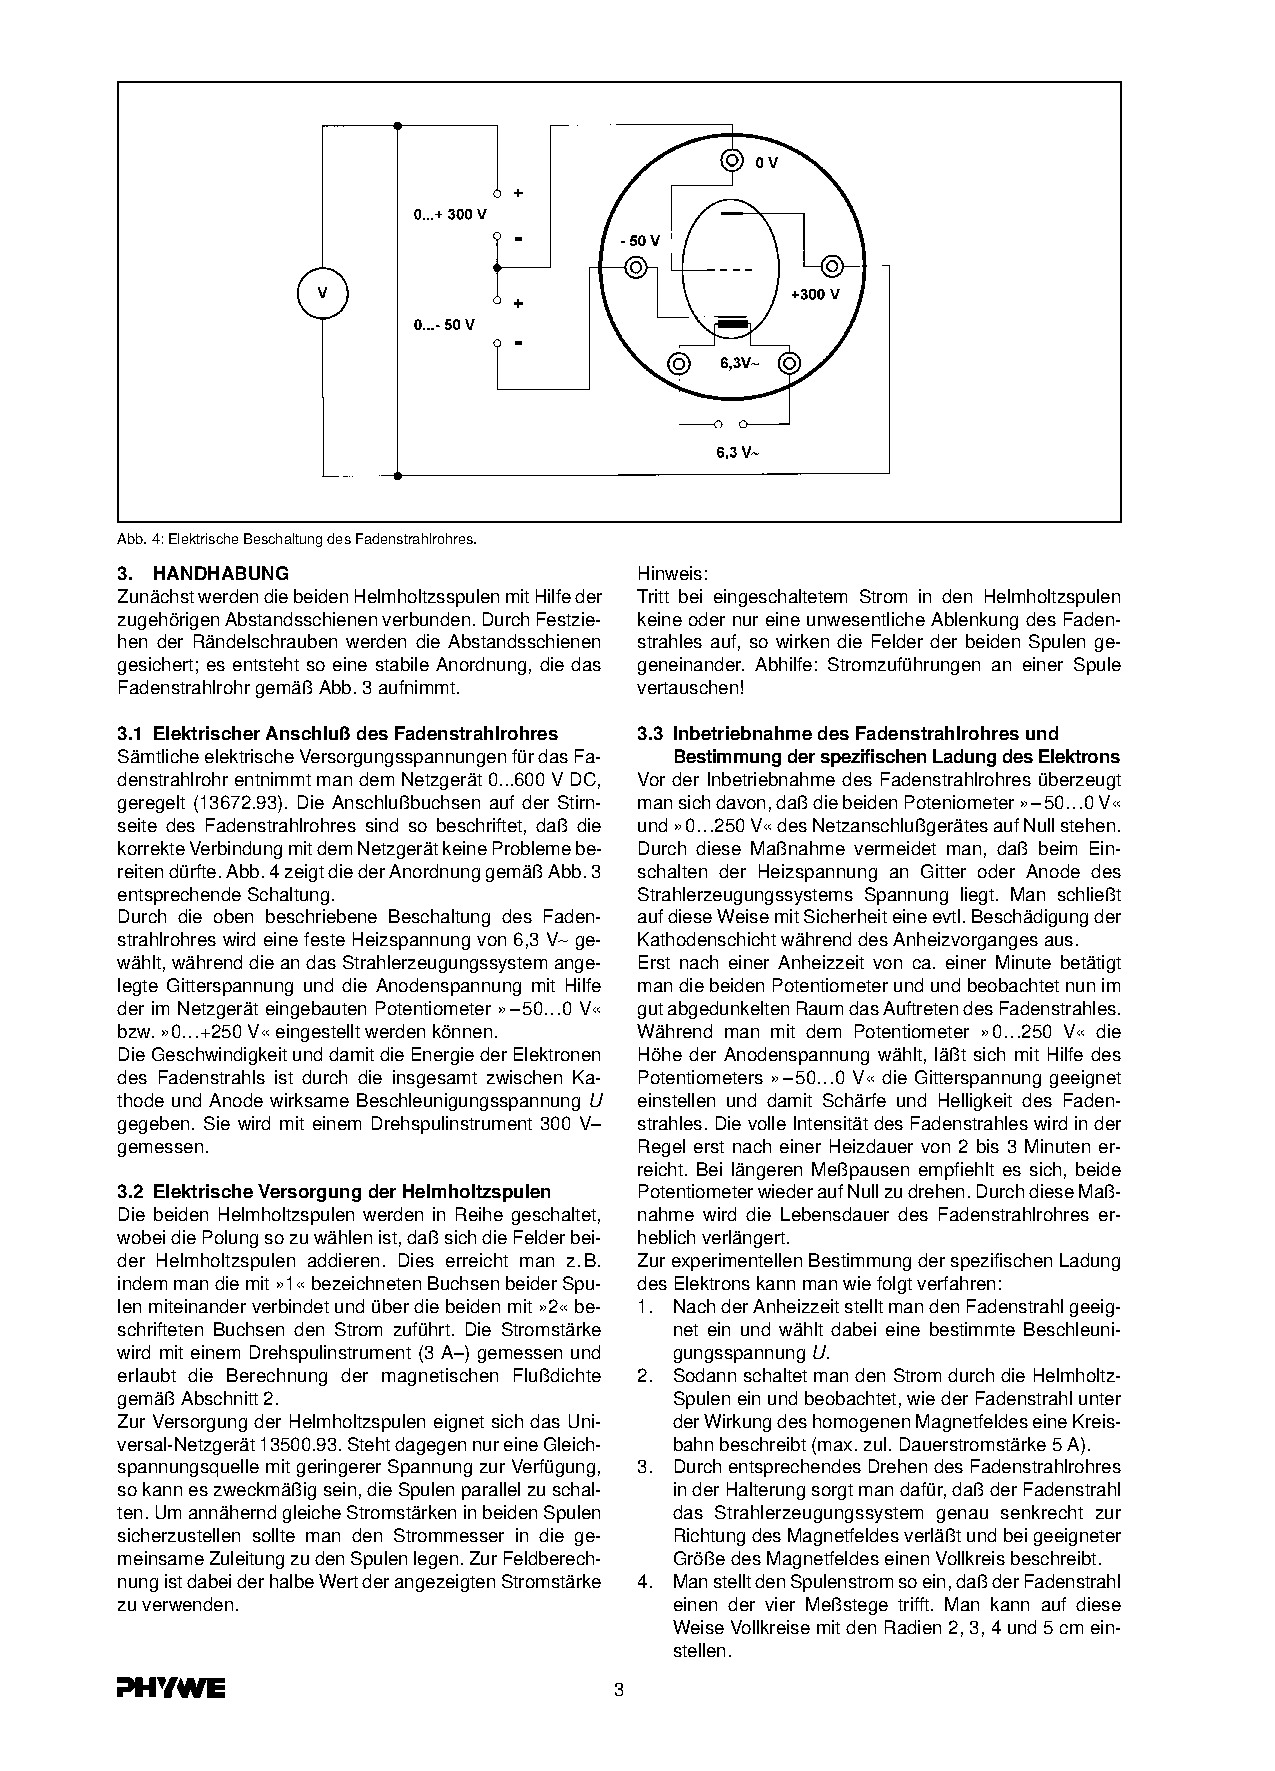
\includegraphics[trim = 10mm 210mm 10mm 10mm, clip, scale = 1]{fadenstrahlrohr.pdf}
  	\caption[Schaltskizze des Fadenstrhlrohrs]{Schaltskizze des Fadenstrhlrohrs\footnotemark}
  \label{fig:aufbau_h}
\end{figure}
\footnotetext{Abbildung entnommen von http://www.atlas.uni-wuppertal.de/\~kind/fadenstrahlrohr\_phywe\_0695900d.pdf am 24.09.2014}

\begin{figure}[H]
\begin{itemize}
\item	6,3V:		Spannung für den Heitzdraht

\item	-50-0 V:	Spannung des Wehneltzylinder

\item	0-300V:		Beschleunigungsspannung
\end{itemize}
\end{figure}

Schaltskizze der Elektronenbeugungsröhre zur Bestimmung der Gitterkonstanten von Graphit.

\begin{figure}[H] 
  \centering
    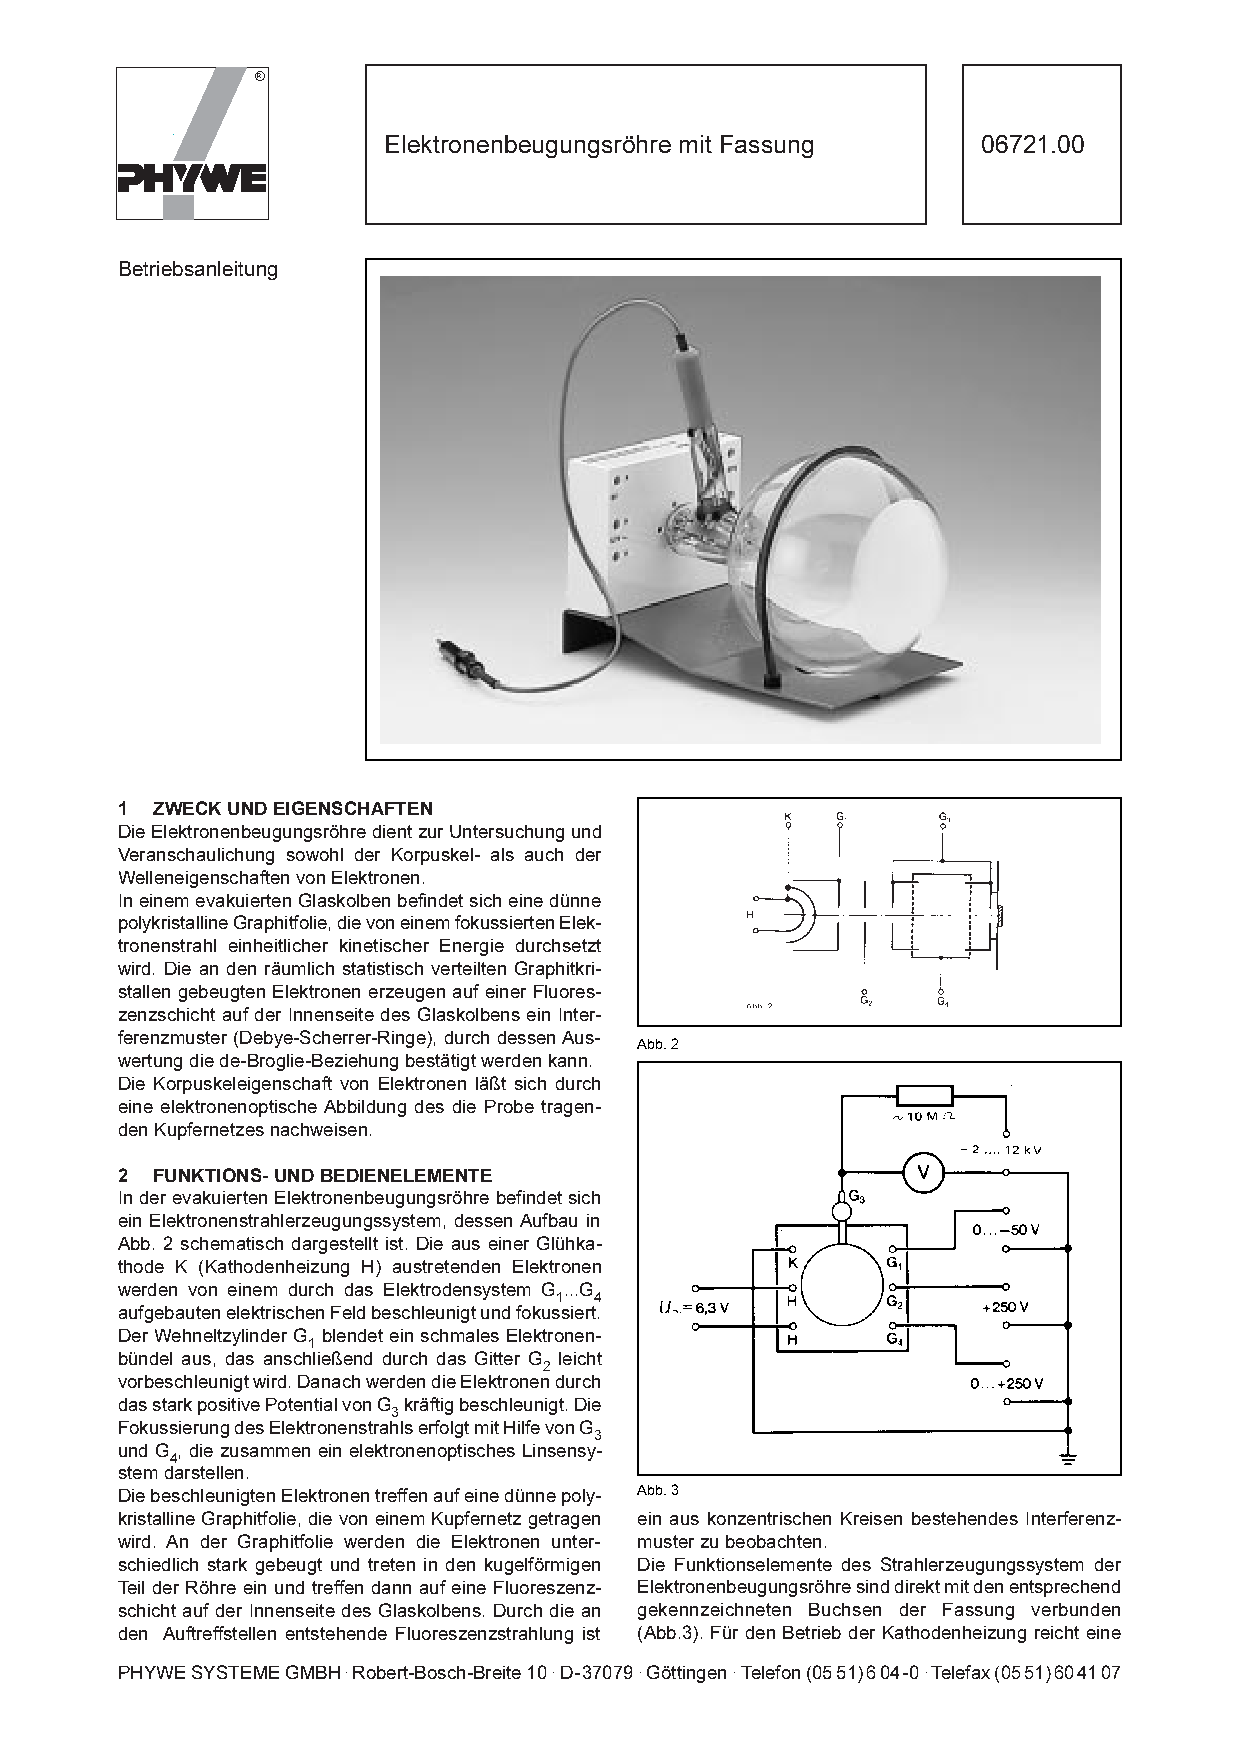
\includegraphics[trim = 105mm 47mm 10mm 178mm, clip, scale = 1]{beugungsroehre.pdf}
  	\caption[Schaltskizze der Elektronenbeugungsröhre]{Schaltskizze der Elektronenbeugungsröhre\footnotemark}
  \label{fig:aufbau_h}
\end{figure}
\footnotetext{Abbildung entnommen von http://www.atlas.uni-wuppertal.de/\~kind/beugungsroehre\_phywe\_0672100d.pdf am 24.09.2014}

\begin{figure}[H]
\begin{itemize}
\item	H:		Kathodenheizung 

\item	K:		Glühkathode

\item	G$_1$:	Wehneltzylinder 

\item	G$_2$:	Gitter zur Vorbeschleunigung

\item	G$_3$:	Beschleunigungsgitter

\item	G$_4$:	Gitter zur Fokussierung
\end{itemize}
\end{figure}

Das Netzgerät, dass für beide Versuchsaufbauten benötigt wird.

\begin{figure}[H] 
  \centering
    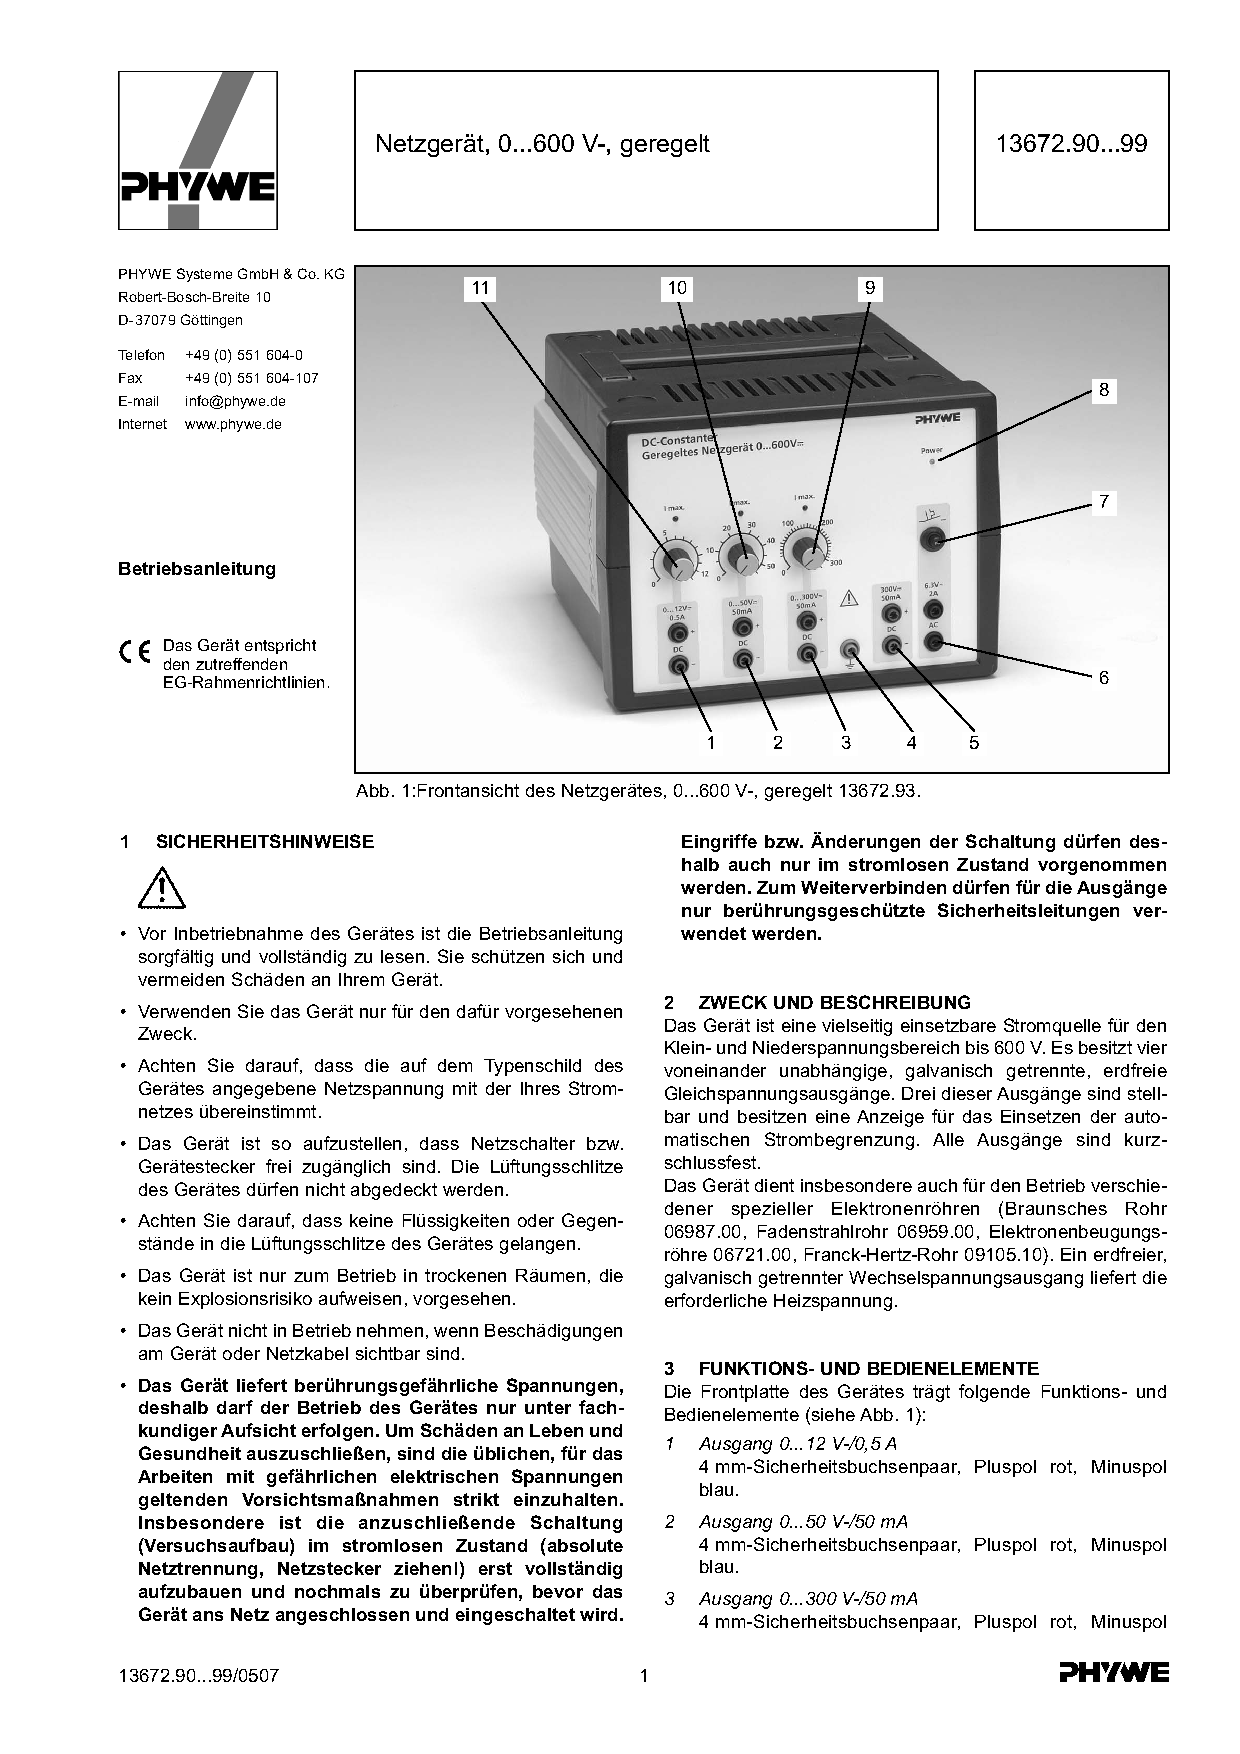
\includegraphics[trim = 60mm 165mm 10mm 40mm, clip, scale = 1]{netzteil.pdf}
  	\caption[Abbild des Netzgerätes]{Abbild des Netzgerätes\footnotemark}
  \label{fig:aufbau_h}
\end{figure}
\footnotetext{Abbildung entnommen von http://www.atlas.uni-wuppertal.de/\~kind/phywe\_600V\_netzteil\_1367293d.pdf am 24.09.2014}

\begin{enumerate}
\item	Ausgang 0-12V-/0,5A

\item	Ausgang 0-50V-/50mA

\item	Ausgang 0-300V-/50mA

\item	Anschluss 'Erde'

\item	Ausgang 300V-/50mA

\item	Ausgang 6,3V\~/2A

\item	Überstromschutzschalter für Ausgang 6,3V

\item	Einschaltkontrollleuchte

\item	Stellknopf für Ausgang 0-300V, rote Leuchtdiode zur Anzeige der Strombegrenzung

\item	Stellknopf für Ausgang 0-50V, rote Leuchtdiode zur Anzeige der Strombegrenzung

\item	Stellknopf für Ausgang 0-12V, rote Leuchtdiode zur Anzeige der Strombegrenzung
\end{enumerate}

\section{Bestimmung der spezifischen Masse $\frac{e}{m}$}
%kurz das ziel dieses versuchsteiles ansprechen, damit keine zwei überschriften direkt übereinander stehen!
%bei schwierigeren versuchen kann auch der theoretische hintergrund erläutert werden. (mit formeln, herleitungen und erklärungen)
Ziel der Messung ist die Bestimmung der spezifischen Ladung $\frac{e}{m}$ des Elektrons mithilfe eines Fadenstrahlrohres.

\subsection{Versuchsaufbau}
%skizze zum versuchsaufbau (oder foto) einfügen,   es muss erklärt werden wie das ganze funktioniert und welche speziellen einstellungen verwendet wurden (z.b. welche knöpfe an den geräten für die messung verdreht wurden)

\begin{figure}[H] 
  \centering
    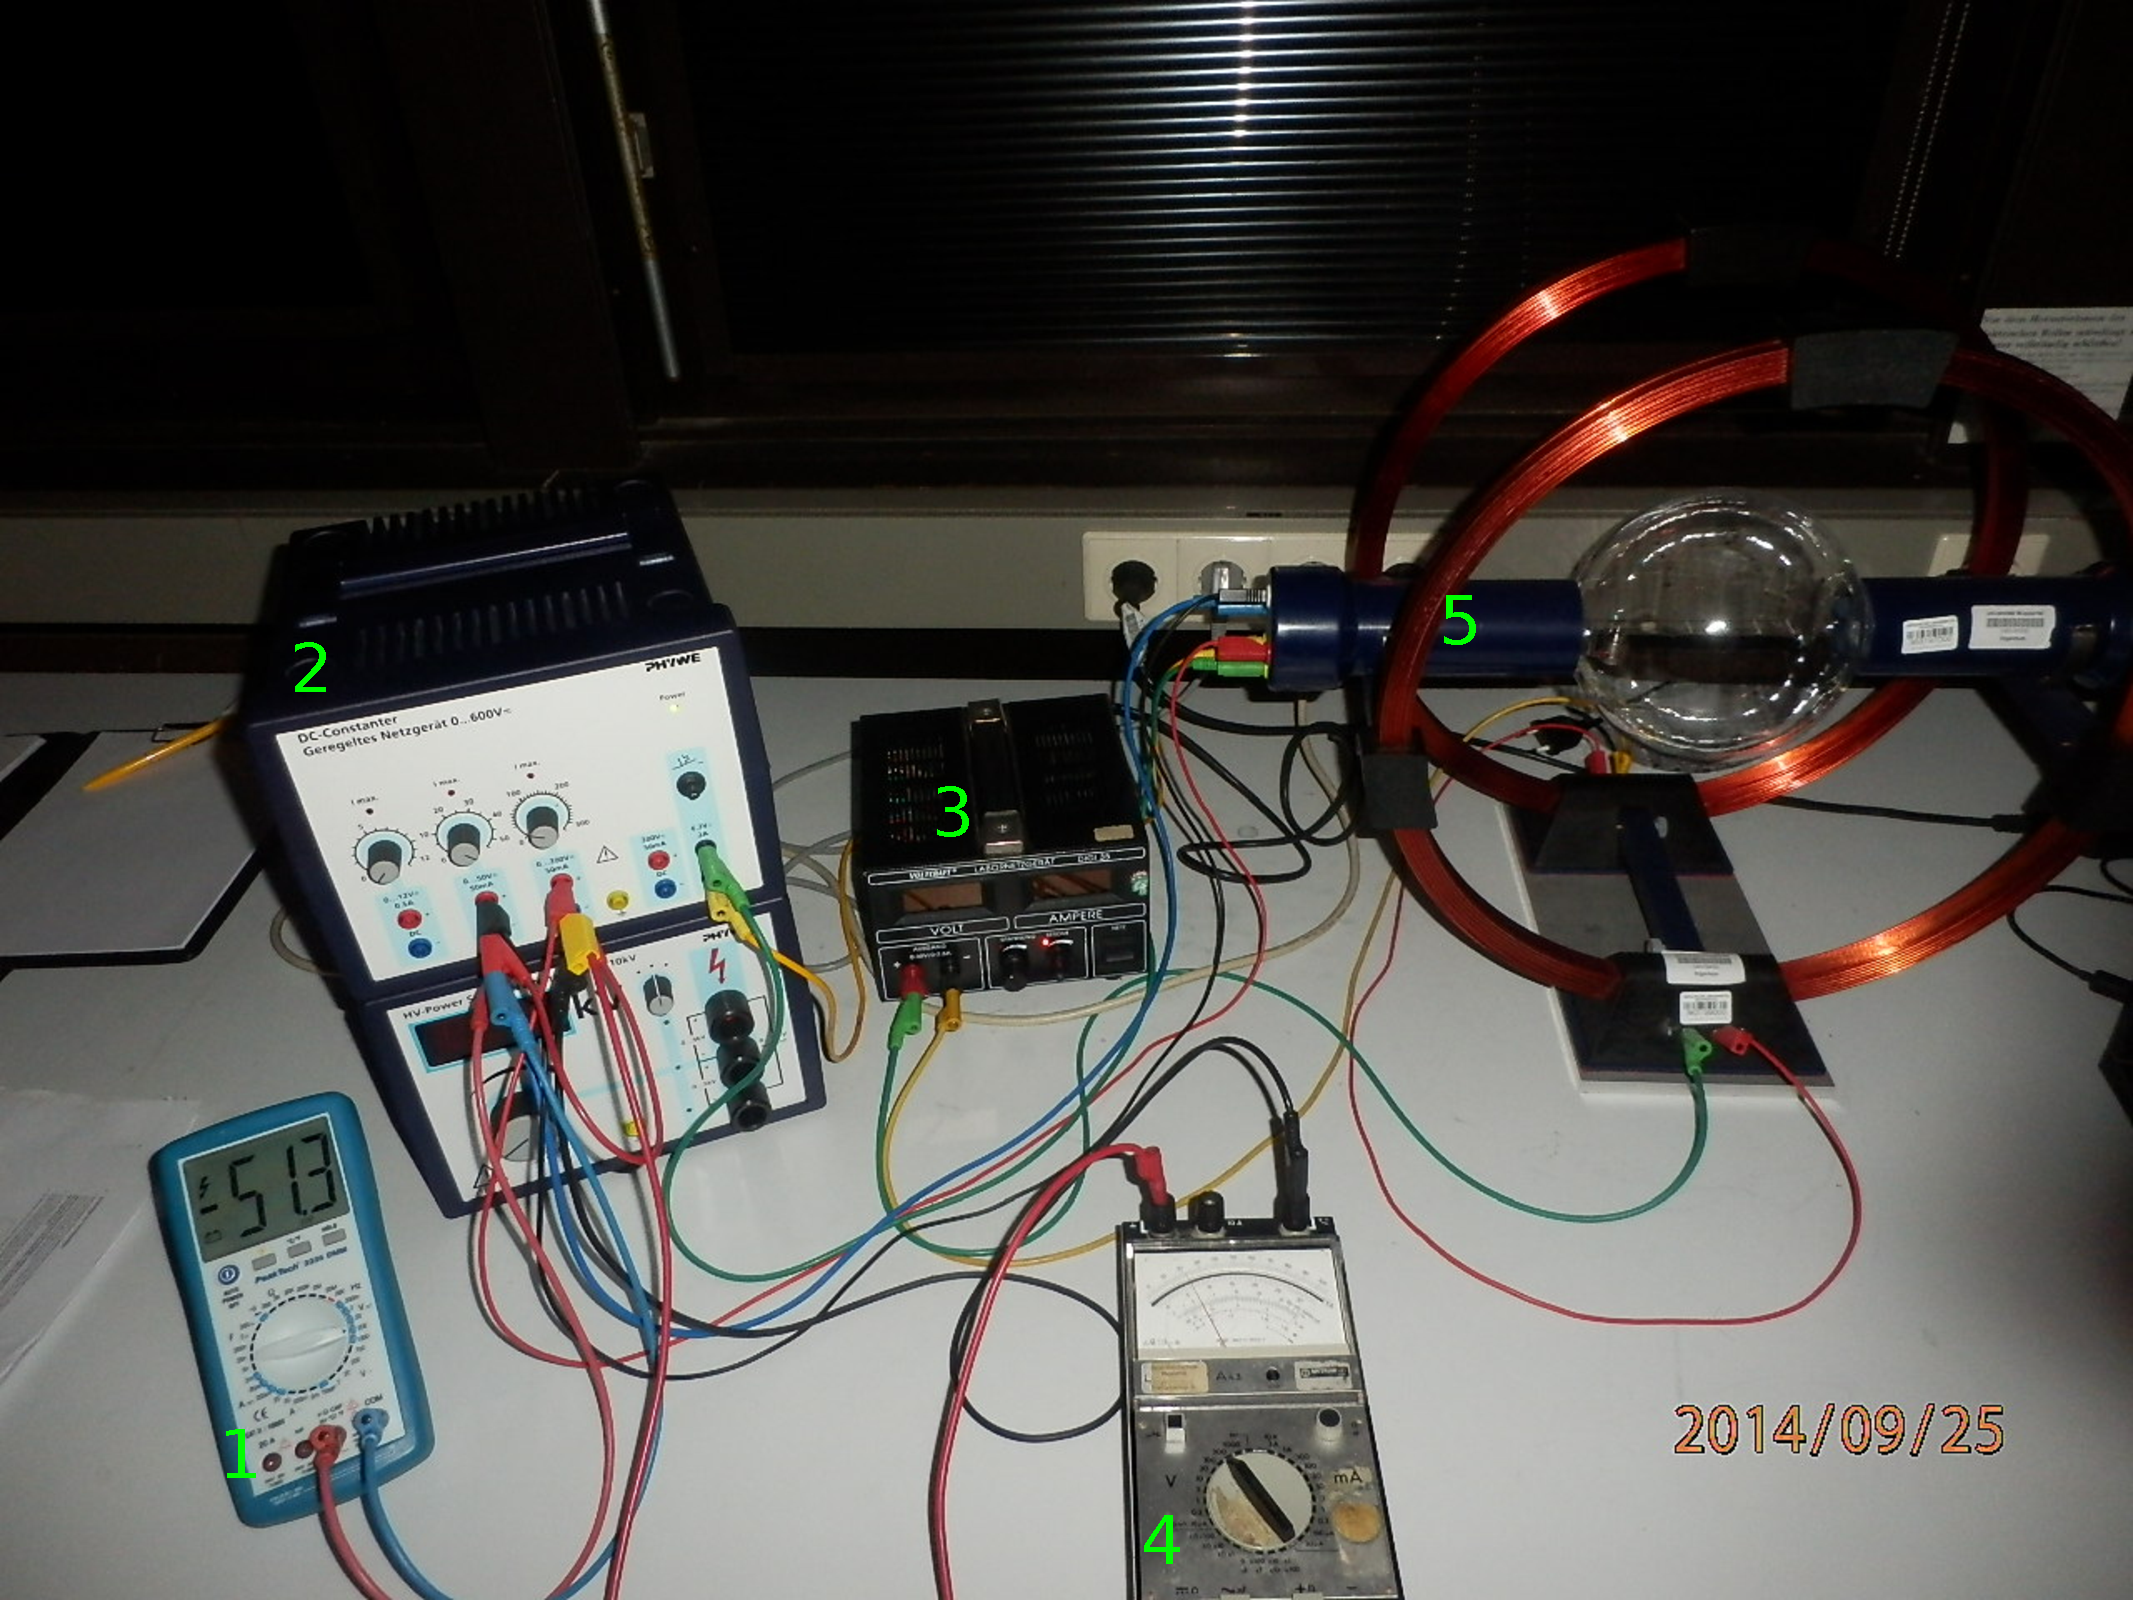
\includegraphics[scale = 0.3]{aufbau_h.pdf}
  	\caption[Abbildung des Versuchsaufbaus zur Bestimmung der spezifischen Ladung von Elektronen]{Abbildung des Versuchsaufbaus zur Bestimmung der spezifischen Ladung von Elektronen}
  \label{fig:aufbau_h}
\end{figure}

\begin{figure}
\begin{enumerate}
\item	DMM zur Messung der Gitterspannung

\item	Netzgerät zur Versorgung der Fadenstrahlrohres

\item	Netzgerät zur Versorgung der Helmholtzspule

\item	Unigor zum messen der Beschleunigungsspannung

\item	Fadenstrahlrohr und Helmholtzspule
\end{enumerate}
\end{figure}


\subsection{Versuchsdurchführung}
%erklären, !was! wir machen, !warum! wir das machen und mit welchem ziel
%(wichtig) präzize erklären, wie bei dem versuch vorgegangen und was gemacht wurde
Zuerst werden die Helmholtzspulen in Reihe an ein Netzgerät angeschlossen, um sicherzugehen, dass durch beide Spulen der selbe Strom fließt. Es muss darauf geachtet werden, dass der Strom in beiden Spulen in die gleiche Richtung fließt, da sonst kein homogenes Magnetfeld zwischen den Spulen entsteht. Der Spulenstrom kann an der Digitalanzeige des Netzgerätes abgelesen und an einem Potentiometer verändert werden. Die Braunsche Röhre wird nach dem Schaltbild in der Versuchsanleitung\footnote{vgl. http://www.atlas.uni-wuppertal.de/
$\sim$kind/fadenstralrohr\_phywe\_0695900d.pdf Seite 3 Abb. 4} an ein weiteres Netzgerät\footnote{vgl. http://www.atlas.uni-wuppertal.de/$\sim$kind/phywe\_600V\_netzteil\_1367293d.pdf}, welches mehrere Ausgänge hat, angeschlossen. Auf dem folgenden Bild ist der schematische Aufbau einer Braunschen Röhre abgebildet.
%bitte das Foto mit dem Schaltbild für die Braunsche Röhre einfügen
In der Mitte zwischen Wehnelt-Zylinder und Anode befindet sich das geerdete Gitter. Parallel zum Gitter und der Anode wird das Unigor (Strom- und Spannungsmessgerät) zur Messung der Beschleunigungsspannung angeschlossen, zur Überprüfung der Spannung zwischen Wehnelt-Zylinder und dem Gitter wird ein DMM parallel geschaltet. Die Spannungen zwischen Gitter und Anode, sowie zwischen Gitter und Wehnelt-Zylinder können am Netzgerät mit entsprechenden Potentiometern eingestellt werden. Die Spannung, welche am Wehnelt-Zylinder anliegt hat neben der Beschleunigung der Elektronen nach Austritt aus der Öffnung den Effekt, den Elektronenstrahl zu fokussieren. Deshalb ist es sinnvoll die Spannung am Wehnelt-Zylinder während des gesamten Versuchsteils konstant zu halten. Für verschiedene Beschleunigungsspannungen und verschiedene Spulenströme soll nun an einer im Fadenstrahlrohr vormontierten Metallleiter der Radius des Elektronenstrahls bestimmt werden (D = (4,6,8,10)cm). Aus dem Durchmesser, den angelegten Spannungen und dem Spulenstrom wird dann die spezifische Ladung $\frac{e}{m}$ errechnet.
\subsection{Verwendete Formeln}
%eine legende kann angefertigt werden, die selbstverständlichen buchstaben müssen nicht extra erklärt werden
%mit knappen erklärungen die !verwendeten! formeln, sowie die zugehörige fehlerrechnung einfügen.

\subsection{Messergebnisse}
%die messwerte in !übersichtlichen! tabellen angegeben
%zu viele kleine tabellen in große tabellen überführen!
%zu große tabellen mit dem [scale]-befehl scalieren oder (falls zu lang) in zwei kleinere tabellen aufteilen
%(wichtig) vor !jeder! tabelle sagen, was gemessen wurde und wie die fehler gewählt wurden und ausreichend !erklären!, !warum! wir unsere fehler grade so gewählt haben

In der folgenden Tabelle sind die Materialeigenschaften, die zur Bestimmung des Magnetfeldes der Helmholtzspulen notwendig sind angegeben. Die Wert wurden als Fehlerlos angenommen, da so in der Versuchsbeschreibung angegeben.

\begin{table}[htbp]
\caption{Materialeigneschaften der Versuchsaufbaus, zur Bestimmung des Magnetfeldes der Helmholzspulen}
\begin{center}
\begin{tabular}{|l|l|l|}
\hline
Materialeigenschaften &  &  \\ \hline
$\mu_0$/(tm/A) & Windungsanzahl & Spulenradius/m \\ \hline
\multicolumn{1}{|r|}{0,000001256} & \multicolumn{1}{r|}{154} & \multicolumn{1}{r|}{0,2} \\ \hline
\end{tabular}
\end{center}
\label{tab:1_m}
\end{table}



In der folgende Tabelle befinden sich die Daten, der ersten bis dritten Messung zur spezifischen Ladung von Elektronen. Der Fehler der Zylinderspannung wurde mit 1,5\% auf dem Unigor angegeben, der Fehler des Radius wurde mit 1\% angegeben, die anderen Fehler wurden alle mit der Ableseungenauigkeit angenommen, bei Schwankungen der Anzeige wurde noch die Hälfte der Schwankungsintervalls dazu addiert.

\begin{table}[H]
\caption{Messdaten der ersten bis dritten Messreihe.}
\begin{center}
\begin{tabular}{|r|r|r|r|r|r|}
\hline
\multicolumn{1}{|l|}{Strom/A} & \multicolumn{1}{l|}{Fehler/A} & \multicolumn{1}{l|}{Zylinder Spannung/V} & \multicolumn{1}{l|}{Fehler/V} & \multicolumn{1}{l|}{} & \multicolumn{1}{l|}{} \\ \hline
1,5 & 0,01 & 51,2 & 0,2 & \multicolumn{1}{l|}{} & \multicolumn{1}{l|}{} \\ \hline
\multicolumn{1}{|l|}{Spannung/V} & \multicolumn{1}{l|}{Fehler/V} & \multicolumn{1}{l|}{Beschleunigungsspannung/V} & \multicolumn{1}{l|}{Fehler/V} & \multicolumn{1}{l|}{Radius/m} & \multicolumn{1}{l|}{Fehler/m} \\ \hline
15,0 & 0,2 & 66,2 & 0,3 & 0,0200 & 0,0002 \\ \hline
36,0 & 0,5 & 87,2 & 0,6 & 0,0300 & 0,0003 \\ \hline
105 & 2 & 156 & 2 & 0,0400 & 0,0004 \\ \hline
189 & 3 & 240 & 3 & 0,0500 & 0,0005 \\ \hline \hline
\multicolumn{1}{|l|}{Strom/A} & \multicolumn{1}{l|}{Fehler/A} & \multicolumn{1}{l|}{Zylinder Spannung/V} & \multicolumn{1}{l|}{Fehler/V} & \multicolumn{1}{l|}{} & \multicolumn{1}{l|}{} \\ \hline
1,7 & 0,01 & 51,2 & 0,2 & \multicolumn{1}{l|}{} & \multicolumn{1}{l|}{} \\ \hline
\multicolumn{1}{|l|}{Spannung/V} & \multicolumn{1}{l|}{Fehler/V} & \multicolumn{1}{l|}{Beschleunigungsspannung/V} & \multicolumn{1}{l|}{Fehler/V} & \multicolumn{1}{l|}{Radius/m} & \multicolumn{1}{l|}{Fehler/m} \\ \hline
30,0 & 0,5 & 81 & 0,5 & 0,0200 & 0,0002 \\ \hline
65 & 1 & 116 & 1 & 0,0300 & 0,0003 \\ \hline
145 & 2 & 196 & 2 & 0,0400 & 0,0004 \\ \hline
259 & 4 & 310 & 4 & 0,0500 & 0,0005 \\ \hline \hline
\multicolumn{1}{|l|}{Strom/A} & \multicolumn{1}{l|}{Fehler/A} & \multicolumn{1}{l|}{Zylinder Spannung/V} & \multicolumn{1}{l|}{Fehler/V} & \multicolumn{1}{l|}{} & \multicolumn{1}{l|}{} \\ \hline
2 & 0,01 & 51,2 & 0,2 & \multicolumn{1}{l|}{} & \multicolumn{1}{l|}{} \\ \hline
\multicolumn{1}{|l|}{Spannung/V} & \multicolumn{1}{l|}{Fehler/V} & \multicolumn{1}{l|}{Beschleunigungsspannung/V} & \multicolumn{1}{l|}{Fehler/V} & \multicolumn{1}{l|}{Radius/m} & \multicolumn{1}{l|}{Fehler/m} \\ \hline
45,0 & 0,7 & 96,2 & 0,7 & 0,0200 & 0,0002 \\ \hline
100 & 2 & 151 & 2 & 0,0300 & 0,0003 \\ \hline
220 & 3 & 271 & 3 & 0,0400 & 0,0004 \\ \hline
\end{tabular}
\end{center}
\label{tab:1_1}
\end{table}




\subsection{Auswertung}
%zuerst !alle! errechneten werte entweder in ganzen sätzen aufzählen, oder in tabellen (übersichtlicher) dargestellen, sowie auf die verwendeten formeln verweisen (die referenzierung der formel kann in der überschrift stehen)
%kurz erwähnen (vor der tabelle), warum wir das ganze ausrechnen bzw. was wir dort ausrechnen
%danach histogramme und plots erstellen, wobei wenn möglich funktionen durch die plots gelegt werden (zur not können auch splines benutzt werden, was aber angegeben werden muss)
%bei fits immer die funktion und das reduzierte chiquadrat mit angegeben, wobei auf verständlichkeit beim entziffern der zehnerpotenzen geachtet werden muss z.b. f(x)=(wert+-fehler)\cdot10^{irgendeine zahl}\cdot x + (wert+-fehler)\cdot10^{irgendeine zahl}
%bei jedem fit erklären, nach welchem zusammenhang gefittet wurde und warum!
%bei plots darauf achten, dass die achsenbeschriftung (auch die tics) die richtige größe haben und die legende im plot nicht die messwerte verdeckt
%kurz die aufgabenstellung abgehandeln

Aus den Gemessenen Daten (Tabelle \ref{tab:1_1}) soll die spezifische Ladung von Elektronen bestimmt werde. Dafür wurde zu erste das Magnetfeld der Helmholzspulen aus dem Strom und den Materialeigenschaften (Tabelle \ref{tab:1_m}) nach Gleichung ?? und der Fehler nach Gleichung ??  bestimmt. Es ergaben sich die folgenden Werte.

\begin{table}[htbp]
\caption{Magnetfelder der drei Messungen}
\begin{center}
\begin{tabular}{|r|r|r|}
\hline
\multicolumn{1}{|l|}{Messung} & \multicolumn{1}{l|}{Magnetfeld/T$\cdot 10^{-6}$} & \multicolumn{1}{l|}{Fehler/T$\cdot 10^{-6}$} \\ \hline
1 & 1176 & 7 \\ \hline
2 & 1038 & 7 \\ \hline
3 & 1384 & 7 \\ \hline
\end{tabular}
\end{center}
\label{tab:aus_b}
\end{table}

Mit Gleichung ?? wurden dann die spezifische Ladung von Elektronen bestimmt, der Fehler wurde mit Gleichung ?? berechnet.

\begin{table}[htbp]
\caption{Spezifische Ladung von Elektronen für verschiedene Radien und Beschleunigungsspannungen}
\begin{center}
\begin{tabular}{|r|r|}
\hline
\multicolumn{1}{|l|}{Messung 1.} & \multicolumn{1}{l|}{} \\ \hline
\multicolumn{1}{|l|}{e/m/($10^{11}$As/kg)} & \multicolumn{1}{l|}{Fehler/($10^{11}$As/kg)} \\ \hline
2,93 & 0,07 \\ \hline
1,87 & 0,05 \\ \hline
1,77 & 0,05 \\ \hline
1,79 & 0,05 \\ \hline \hline
\multicolumn{1}{|l|}{Messung 2.} & \multicolumn{1}{l|}{} \\ \hline
\multicolumn{1}{|l|}{e/m/($10^{11}$As/kg)} & \multicolumn{1}{l|}{Fehler/($10^{11}$As/kg)} \\ \hline
3,07 & 0,08 \\ \hline
1,80 & 0,04 \\ \hline
1,81 & 0,05 \\ \hline
1,78 & 0,05 \\ \hline \hline
\multicolumn{1}{|l|}{Messung 3.} & \multicolumn{1}{l|}{} \\ \hline
\multicolumn{1}{|l|}{e/m/($10^{11}$As/kg)} & \multicolumn{1}{l|}{Fehler/($10^{11}$As/kg)} \\ \hline
2,51 & 0,06 \\ \hline
1,75 & 0,04 \\ \hline
1,77 & 0,05 \\ \hline
\end{tabular}
\end{center}
\label{tab:aus_e/m}
\end{table}

Gemittelt ergibt sich ein Wert von \unit{(1,79 $\pm$0,01)$\cdot 10^{11}$}[$\frac{\text{As}}{\text{kg}}$], dabei wurden der erste Wert jeder Messung nicht mit einbezogen, da die Gitterspannung und die Beschleunigungsspannung zu nach bei einander liegen, wodurch das Ergebnis stark verfälscht wurde.

\subsection{Diskussion}
%(immer) die gemessenen werte und die bestimmten werte über die messfehler mit literaturwerten oder untereinander vergleichen
%in welchem fehlerintervall des messwertes liegt der literaturwert oder der vergleichswert?
%wie ist der relative anteil des fehlers am messwert und damit die qualität unserer messung?
%in einem satz erklären, wie gut unser fehler und damit unsere messung ist
%kurz erläutern, wie systematische fehler unsere messung beeinflusst haben könnten
%(wichtig) zum schluss ansprechen, in wie weit die ergebnisse mit der theoretischen vorhersage übereinstimmen
%--------------------------------------------------------------------------------------------
%falls tabellen mit den messwerten zu lang werden, kann die section mit den messwerten auch hinter der diskussion angefügt bzw. eine section mit dem anhang eingefügt werden.

Es wurde eine spezifische Ladung von \unit{1,76 $\cdot 10^{11}$}[$\frac{As}{kg}$] für Elektronen erwartet, der von uns bestimmte Wert liegt bei \unit{(1,79 $\pm$0,03)$\cdot 10^{11}$}[$\frac{\text{As}}{\text{kg}}$]. Der Anteil der des Fehlers am Messwert liegt bei 1,83\%. Die prozentuale Abweichung vom Literaturwert beträgt 1,77\%, was für eine guter Wert ist. Der Literaturwert liegt im ersten Fehlerintervall des bestimmten Wertes. Eine Relativeistische Betrachtung ist nicht nötig, da sich die Elektronen maximal mit 3,5\% der Lichtgeschwindigkeit bewegen.

\section{Beugung von Elektronenstrahlen, Verifikation der DeBroglie-Beziehung}
%kurz das ziel dieses versuchsteiles ansprechen, damit keine zwei überschriften direkt übereinander stehen!
%bei schwierigeren versuchen kann auch der theoretische hintergrund erläutert werden. (mit formeln, herleitungen und erklärungen)
Ziel des Versuchs ist die Bestimmung der Gitterkonstanten $d_1$ und $d_2$ einer Graphitschicht anhand des Interferenzmusters, welches durch den Beschuss mit Elektronen entsteht. Dabei sollen relativistische Effekte berücksichtigt werden.
\subsection{Versuchsaufbau}
%skizze zum versuchsaufbau (oder foto) einfügen,   es muss erklärt werden wie das ganze funktioniert und welche speziellen einstellungen verwendet wurden (z.b. welche knöpfe an den geräten für die messung verdreht wurden)
\subsection{Versuchsdurchführung}
%erklären, !was! wir machen, !warum! wir das machen und mit welchem ziel
%(wichtig) präzize erklären, wie bei dem versuch vorgegangen und was gemacht wurde
Zuerst schalten wir die Elektronenbeugungsröhre gemäß des Schaltbildes in der Versuchsbeschreibung\footnote{vgl. http://www.atlas.uni-wuppertal.de/
$\sim$kind/beugungsroehre\_phywe\_0672100d.pdf Seite 1 Abb. 2 und 3}. Die Spannung am Wehnelt-Zylinder ist für die Fokussierung des Elektronenstrahls verantwortlich, weshalb wir diese maximal gewählt haben, die Beschleunigungsspannung der Braunschen Röhre ist dagegen eher unwichtig und wir haben sie deshalb minimal gewählt. Da die Energiezunahme der Elektronen durch die Spannung am Wehnelt-Zylinder im Vergleich zur Energiezunahme durch die dahinter geschaltetete Anodenspannung von 2 bis 12kV zu vernachlässigen ist, wird diese im folgenden nicht weiter berücksichtigt. Die Elektronen erreichen bei einer Spannung von 12kV eine Geschwindigkeit von etwas weniger als 22\% der Lichtgeschwindigkeit. Deshalb ist in diesem Versuchsteil eine relativistische Betrachtung bzw. eine Abschätzung des Fehlers durch relativistische Effekte sinnvoll. Nachdem die Kathode aufgeheizt und die Spannungen angeschaltet sind, kann am Schirm der Elektronenbeugungsröhre das Interferenzmuster, welches sich aus der Bragg-Gleichung ergibt, beobachtet und mit der hinter dem Schirm angeklebten Millimeterfolie vermessen werden\footnote{Herleitung der Bragg-Gleichung/Bedingung für konstruktive Interferenz http://de.wikipedia.org/wiki/Bragg-Gleichung}.
Da die Kristallgitter statistisch angeordnet sind und wir in diesem Versuch nur die ersten Maxima für beide bekannten Gitterkonstanten $d_1$ und $d_2$ untersuchen, können wir über den Durchmesser der am Schirm leuchtenden Kreise, die durch die Interferenz der Elektronen am Kristallgitter entstehen, die Gitterkonstanten experimentell verifizieren und damit die DeBroglie-Beziehung nachweisen.
\subsection{Verwendete Formeln}
%eine legende kann angefertigt werden, die selbstverständlichen buchstaben müssen nicht extra erklärt werden
%mit knappen erklärungen die !verwendeten! formeln, sowie die zugehörige fehlerrechnung einfügen.
\subsection{Messergebnisse}
%die messwerte in !übersichtlichen! tabellen angegeben
%zu viele kleine tabellen in große tabellen überführen!
%zu große tabellen mit dem [scale]-befehl scalieren oder (falls zu lang) in zwei kleinere tabellen aufteilen
%(wichtig) vor !jeder! tabelle sagen, was gemessen wurde und wie die fehler gewählt wurden und ausreichend !erklären!, !warum! wir unsere fehler grade so gewählt haben
\subsection{Auswertung}
%zuerst !alle! errechneten werte entweder in ganzen sätzen aufzählen, oder in tabellen (übersichtlicher) dargestellen, sowie auf die verwendeten formeln verweisen (die referenzierung der formel kann in der überschrift stehen)
%kurz erwähnen (vor der tabelle), warum wir das ganze ausrechnen bzw. was wir dort ausrechnen
%danach histogramme und plots erstellen, wobei wenn möglich funktionen durch die plots gelegt werden (zur not können auch splines benutzt werden, was aber angegeben werden muss)
%bei fits immer die funktion und das reduzierte chiquadrat mit angegeben, wobei auf verständlichkeit beim entziffern der zehnerpotenzen geachtet werden muss z.b. f(x)=(wert+-fehler)\cdot10^{irgendeine zahl}\cdot x + (wert+-fehler)\cdot10^{irgendeine zahl}
%bei jedem fit erklären, nach welchem zusammenhang gefittet wurde und warum!
%bei plots darauf achten, dass die achsenbeschriftung (auch die tics) die richtige größe haben und die legende im plot nicht die messwerte verdeckt
%kurz die aufgabenstellung abgehandeln
\subsection{Diskussion}
%(immer) die gemessenen werte und die bestimmten werte über die messfehler mit literaturwerten oder untereinander vergleichen
%in welchem fehlerintervall des messwertes liegt der literaturwert oder der vergleichswert?
%wie ist der relative anteil des fehlers am messwert und damit die qualität unserer messung?
%in einem satz erklären, wie gut unser fehler und damit unsere messung ist
%kurz erläutern, wie systematische fehler unsere messung beeinflusst haben könnten
%(wichtig) zum schluss ansprechen, in wie weit die ergebnisse mit der theoretischen vorhersage übereinstimmen
%--------------------------------------------------------------------------------------------
%falls tabellen mit den messwerten zu lang werden, kann die section mit den messwerten auch hinter der diskussion angefügt bzw. eine section mit dem anhang eingefügt werden.
\section{Fazit}
%im fazit nochmal alles zusammenfassen und den verlauf der messung abschätzen
%gravierende sytematische probleme bei den messungen nochmal betonen und die wertigkeit unserer ergebnisse einordnen
\end{document}